\PassOptionsToPackage{unicode=true}{hyperref} % options for packages loaded elsewhere
\PassOptionsToPackage{hyphens}{url}
%
\documentclass[]{book}
\usepackage{lmodern}
\usepackage{amssymb,amsmath}
\usepackage{ifxetex,ifluatex}
\usepackage{fixltx2e} % provides \textsubscript
\ifnum 0\ifxetex 1\fi\ifluatex 1\fi=0 % if pdftex
  \usepackage[T1]{fontenc}
  \usepackage[utf8]{inputenc}
  \usepackage{textcomp} % provides euro and other symbols
\else % if luatex or xelatex
  \usepackage{unicode-math}
  \defaultfontfeatures{Ligatures=TeX,Scale=MatchLowercase}
\fi
% use upquote if available, for straight quotes in verbatim environments
\IfFileExists{upquote.sty}{\usepackage{upquote}}{}
% use microtype if available
\IfFileExists{microtype.sty}{%
\usepackage[]{microtype}
\UseMicrotypeSet[protrusion]{basicmath} % disable protrusion for tt fonts
}{}
\IfFileExists{parskip.sty}{%
\usepackage{parskip}
}{% else
\setlength{\parindent}{0pt}
\setlength{\parskip}{6pt plus 2pt minus 1pt}
}
\usepackage{hyperref}
\hypersetup{
            pdftitle={Guidelines for Computational Reproducibility in Economics},
            pdfauthor={ACRE Team},
            pdfborder={0 0 0},
            breaklinks=true}
\urlstyle{same}  % don't use monospace font for urls
\usepackage{longtable,booktabs}
% Fix footnotes in tables (requires footnote package)
\IfFileExists{footnote.sty}{\usepackage{footnote}\makesavenoteenv{longtable}}{}
\usepackage{graphicx,grffile}
\makeatletter
\def\maxwidth{\ifdim\Gin@nat@width>\linewidth\linewidth\else\Gin@nat@width\fi}
\def\maxheight{\ifdim\Gin@nat@height>\textheight\textheight\else\Gin@nat@height\fi}
\makeatother
% Scale images if necessary, so that they will not overflow the page
% margins by default, and it is still possible to overwrite the defaults
% using explicit options in \includegraphics[width, height, ...]{}
\setkeys{Gin}{width=\maxwidth,height=\maxheight,keepaspectratio}
\setlength{\emergencystretch}{3em}  % prevent overfull lines
\providecommand{\tightlist}{%
  \setlength{\itemsep}{0pt}\setlength{\parskip}{0pt}}
\setcounter{secnumdepth}{5}
% Redefines (sub)paragraphs to behave more like sections
\ifx\paragraph\undefined\else
\let\oldparagraph\paragraph
\renewcommand{\paragraph}[1]{\oldparagraph{#1}\mbox{}}
\fi
\ifx\subparagraph\undefined\else
\let\oldsubparagraph\subparagraph
\renewcommand{\subparagraph}[1]{\oldsubparagraph{#1}\mbox{}}
\fi

% set default figure placement to htbp
\makeatletter
\def\fps@figure{htbp}
\makeatother

\usepackage{booktabs}
\usepackage[]{natbib}
\bibliographystyle{apalike}

\title{Guidelines for Computational Reproducibility in Economics}
\author{ACRE Team}
\date{2020-03-25}

\begin{document}
\maketitle

{
\setcounter{tocdepth}{1}
\tableofcontents
}
\hypertarget{section}{%
\chapter*{}\label{section}}
\addcontentsline{toc}{chapter}{}

\begin{verbatim}
                (1)       (2)         (3)        (4)        (5)
              scope --> assess --> improve --> robust --> extend
               ▲         |  |                   ▲
               |         |  |                   |
               |_________|  |___________________|
\end{verbatim}

\protect\hyperlink{scoping}{(1) Scoping}

\protect\hyperlink{assessment}{(2) Assessment}

\protect\hyperlink{improvements}{(3) Improvement}

\protect\hyperlink{robust}{(4) Robustness}

\begin{enumerate}
\def\labelenumi{(\arabic{enumi})}
\setcounter{enumi}{4}
\tightlist
\item
   Extensions

  \protect\hyperlink{improvements}{Outcome-level}

  \protect\hyperlink{paper-level}{Paper-level}

  ☐ Select paper

  \protect\hyperlink{describe-inputs}{☐ Describe inputs}

  \protect\hyperlink{rd}{☐ + Raw data}

  \protect\hyperlink{paper-level}{☐ + Version control}

  \protect\hyperlink{id-analy}{☐ Analytical choices}

  ☐ New method

  \protect\hyperlink{check-acre}{☐ Check ACRE}

  \protect\hyperlink{diagram}{☐ Reproduction diagrams}

  \protect\hyperlink{ad}{☐ + Analysis data}

  \protect\hyperlink{paper-level}{☐ + Documentation}

  \protect\hyperlink{id-type}{☐ Type of choice}

  ☐ New data

  ☐ \protect\hyperlink{verify-rep-mat}{Check Rep.~pkg exists}

  \protect\hyperlink{score}{☐ Reproduction score}

  \protect\hyperlink{ac}{☐ + Analysis code}

  \protect\hyperlink{paper-level}{☐ + Dynamic document}

  \protect\hyperlink{id-val}{☐ Choice value}

  ☐ New data

  \protect\hyperlink{read-summ}{☐ Read paper}

  \protect\hyperlink{dac}{☐ Debug analysis code}

  \protect\hyperlink{paper-level}{☐ + File structure}

  \protect\hyperlink{test-rob}{☐ Justify and test alternatives}

  \protect\hyperlink{declare-estimates}{☐ Declare estimates}

  \protect\hyperlink{dcc}{☐ Debug cleaning code}

  \protect\hyperlink{dcc}{☐ Debug cleaning code}

  \href{https://berkeley.qualtrics.com/jfe/form/SV_3UWe5xu3qjeh0c5}{Record results in Survey 1}

  \href{https://berkeley.qualtrics.com/jfe/form/SV_2gd9Y3XVtjLpZL7}{Record results in Survey 2}

  \href{ADD\%20LINK}{Record results in Survey 3}
\end{enumerate}

\hypertarget{intro}{%
\chapter*{Introduction}\label{intro}}
\addcontentsline{toc}{chapter}{Introduction}

In 2019, the \href{https://www.aeaweb.org/journals/policies/data-code/}{American Economic Association} updated its Data and Code Availability Policy, which now mandates that the AEA Data Editor verifies the reproducibility of all papers before they are accepted by an AEA journal. In addition to the requirements, several \href{https://aeadataeditor.github.io/aea-de-guidance/}{specific recommendations} were produced to facilitate compliance. This change in policy is expected to improve the computational reproducibility of all newly published research, after several studies showed that rates of \emph{computational reproducibility} in economics at large range from alarmingly low \citep{galiani2018make, chang2015economics} to just low \citep{kingi2018reproducibility}.

\emph{Replication}, or the process by which a study's hypotheses and findings are re-examined using different data or different methods (or both) \citep{King95} is an essential part of the scientific process that allows science to be ``self-correcting.'' \emph{Computational reproducibility}, or the ability to reproduce the results, tables, and other figures using the available data, code, and materials, is a precondition for replication. Computational reproducibility is assessed through the process of \emph{reproduction}. At the center of this process is the \emph{reproducer} (you!), a party not involved in the production of the original paper. Reproductions sometimes involve the \emph{original author} (whom we refer to as ``the author'') in cases where additional guidance and materials are needed to execute the process.

This exercise is designed for reproductions performed in economics graduate courses or undergraduate theses, with the goal of providing a common approach, terminology, and standards for conducting reproductions. The goal of reproduction, in general, is to assess and improve the computational reproducibility of published research in a way that facilitates future replication, extension, and collaboration.

This exercise is part of the Accelerating Computational Reproducibility in Economics \href{https://www.bitss.org/ecosystem/acre/}{(ACRE)} project led by the Berkeley Initiative for Transparency in the Social Sciences \href{bitss.org}{(BITSS)} and Prof.~Lars Vilhuber, Data Editor for the journals of the American Economic Association (AEA). ACRE looks to assess, enable, and improve the computational reproducibility of published economics research.

\hypertarget{beyond-binary-judgments}{%
\section*{Beyond binary judgments}\label{beyond-binary-judgments}}
\addcontentsline{toc}{section}{Beyond binary judgments}

Assessments of reproducibility can easily gravitate towards binary assessments that declare an entire paper ``reproducible'' or ``non-reproducible''. These guidelines suggest a more nuanced approach by highlighting two reasons that make binary judgment less relevant.

First, a paper may contain several scientific claims, out of which all can vary in computational reproducibility. Each claim is tested using different methodologies, where results are presented in one or more outputs (like table and figures). Each output will itself contain several specifications. Figure \ref{fig:diagram} illustrates this idea.

\begin{figure}
\centering
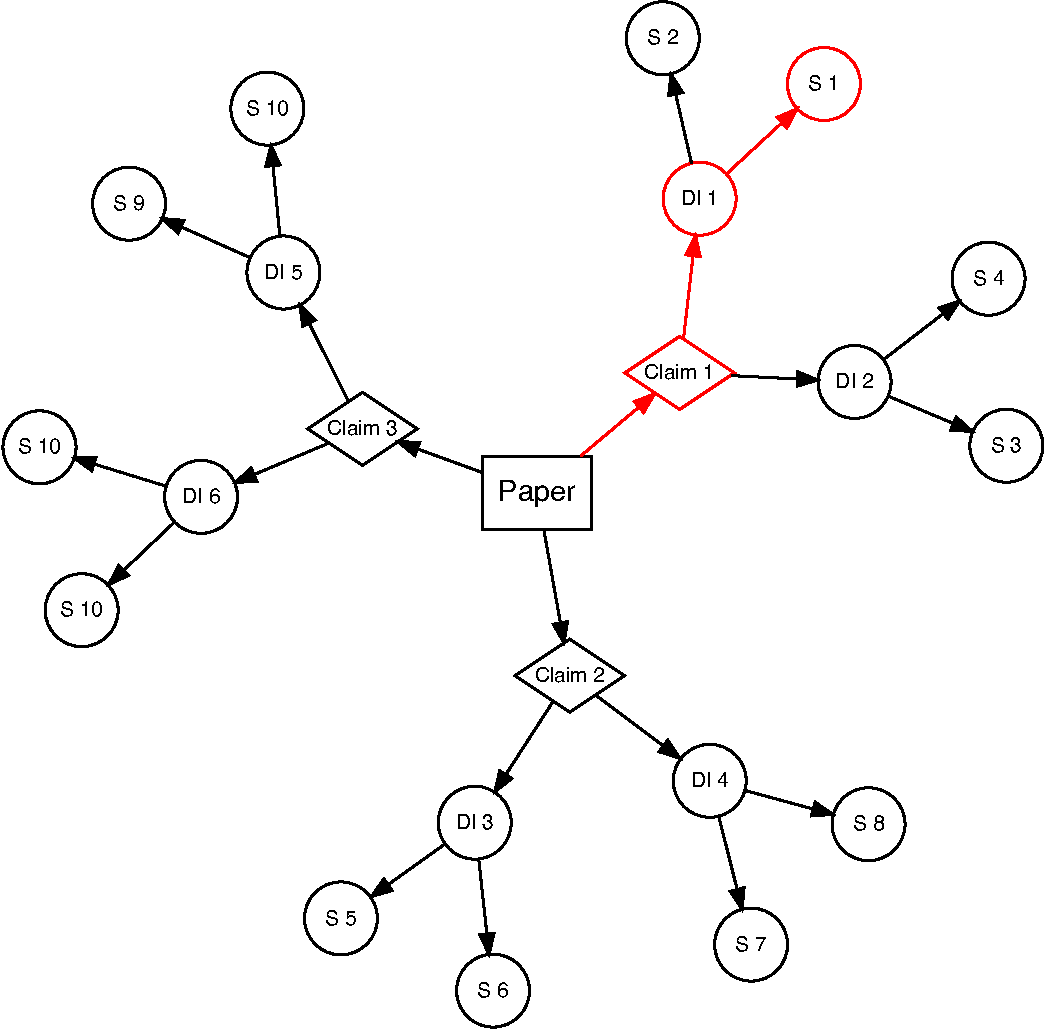
\includegraphics{01-intro_files/figure-latex/diagram-1.pdf}
\caption{\label{fig:diagram}One paper has multiple components to reproduce}
\end{figure}

Second, for a given specification there are several levels of reproducibility, ranging from the absence of any materials to complete reproducibility starting from the raw data. And even for a specific claim-specification, distinguishing the appropriate level can be far more constructive than simple labeling as (ir)reproducible.

Note that the highest level of reproducibility, which requires complete reproducibility starting from raw data, is very demanding and it should not be expected of all published research -- especially before 2019. Instead, this level serves as an aspiration to improve the current reproducibility of research and facilitate the transmission of knowledge in the scientific community.

\hypertarget{stages-of-the-exercise}{%
\section*{Stages of the exercise}\label{stages-of-the-exercise}}
\addcontentsline{toc}{section}{Stages of the exercise}

This reproduction exercise is divided into four stages, corresponding to the first four chapters of these guidelines, with a fifth optional stage :

\begin{enumerate}
\def\labelenumi{\arabic{enumi}.}
\item
  \protect\hyperlink{scoping}{\textbf{Scoping}}, where you (the reproducer) will define the scope of the exercise by declaring a paper and the specific output(s) on which you will focus in the remainder of the exercise;\\
\item
  \protect\hyperlink{assessment}{\textbf{Assessment}}, where you will review and describe in detail the available reproduction package, and assess the current level of computational reproducibility of the selected outputs;
\item
  \protect\hyperlink{improvements}{\textbf{Improvement}}, where you will modify the content and/or the organization of the reproduction package to improve its reproducibility;\\
\item
  \protect\hyperlink{robust}{\textbf{Robustness checks}}, where will assess the quality of selected analytical choices from the paper; and\\
\item
  \textbf{Extension} (if applicable), where you may extend the current paper by including new methodologies or data. This step brings the reproduction exercise a step closer to \emph{replication}.

\begin{verbatim}
     Figure 2: Steps for reproduction

            (1)       (2)         (3)        (4)        (5)
          scope --> assess --> improve --> robust --> extend
           ▲         |  |                   ▲
           |         |  |                   |
           |_________|  |___________________|

 Suggested level of effort:
- Graduate
  research:   5%       10%        5%         10%         70%
- Graduate
  course:    10%       25%       20%         40%         5%
- Undergrad.
  thesis:    10%       30%       40%         20%         0%
\end{verbatim}
\end{enumerate}

Figure 2 depicts suggested levels of effort for each stage of the exercise depending on the context in which the reproducer is performing a reproduction. This process need not be chronologically linear, e.g., the reproducer may realize that the scope of a reproduction is too ambitious and switch to a less intensive reproduction. Later in the exercise, the reproducer can also begin testing different specifications for robustness while also assessing a paper's level of reproducibility.

\hypertarget{recording-the-results-of-the-exercise}{%
\section*{Recording the results of the exercise}\label{recording-the-results-of-the-exercise}}
\addcontentsline{toc}{section}{Recording the results of the exercise}

You will be asked to record the results of their reproduction progress through each stage.

At \emph{Stage 1:\protect\hyperlink{scoping}{Scoping}}, complete \textbf{\href{https://berkeley.qualtrics.com/jfe/form/SV_8hLHNI6LGSYchEN}{Survey 1}}, where you will declare the paper of choice and the specific output(s) on which you will focus for the remainder of the exercise. This step may also involve writing a brief 1-2 page summary of the paper (confirm this with your instructor).

At \emph{Stage 2: \protect\hyperlink{assessment}{Assessment}}, you will inspect the paper's reproduction package (raw data, analysis data, and code), connect the output to reproduce with its inputs, and assign a reproducibility score to each output. At \emph{Stage 3: \protect\hyperlink{improvements}{Improvement}}, you will try to improve the reproducibility of the selected outputs by adding missing files and documentation, and will report potential changes in the level of reproducibility. Use \textbf{Survey 2} to record your work at Stages 2 and 3.

At \emph{Stage 4: \protect\hyperlink{robust}{Robustness Checks}} you will assess different analytical choices and test possible variations. Use \textbf{Survey 3} to record your work at this stage.

\hypertarget{scoping}{%
\chapter{Scoping}\label{scoping}}

In this stage, you will choose a paper to reproduce or be assigned one, verify that the paper has some reproduction materials, and if materials are available, you will read the paper and declare the scope of the reproduction exercise. \textbf{\emph{Use \href{https://berkeley.qualtrics.com/jfe/form/SV_3UWe5xu3qjeh0c5}{Survey 1} to record your work for this stage.}} In this stage, \emph{you are not expected to review the reproduction materials in detail}, as you will dedicate most of your time to this in the later stages of the exercise. You can expect to spend between 1-3 days in the Scoping stage.

\hypertarget{select-a-candidate-paper-or-be-assigned-one.}{%
\section{Select a candidate paper or be assigned one.}\label{select-a-candidate-paper-or-be-assigned-one.}}

Ideally, you should select your candidate paper without previously exploring the availability of materials. In the following sections (\ref{check-acre} and \ref{verify-rep-mat}) these guidelines will show you how to inspect the feasibility of starting a reproduction exercise in your candidate paper. If there are not enough materials to pursue a reproduction, you will be asked to create a short entry in the ACRE platform (\textless{}15 minutes) and select a new candidate paper.

Repeat this step until you have found a paper with a reproduction package -- this will be your \textbf{\emph{declared paper}} and you will try to reproduce it in the remainder of the ACRE exercise. Do not invest time in doing a detailed read of any paper until you are sure that it is your declared paper.

\hypertarget{check-acre}{%
\section{Check records on the ACRE platform.}\label{check-acre}}

Check the \href{ADD\%20LINK}{ACRE database} for previous assessments of your candidate paper. If there are previous entries, you will see a brief report card with the following information:

\begin{quote}
\textbf{Title:} Sample Title\\
\textbf{Authors:} Jane Doe \& John Doe\\
\textbf{Original Reproduction Package Available:} URL/No\\
{[}If ``No''{]} \textbf{Contacted Authors?:} Yes/No\\
{[}If ``Yes(contacted)''{]} \textbf{Type of Response:} Categories (6).\\
\textbf{Additional Reproduction Packages:} Number (eg., 2)\\
\textbf{Authors Available for Further Questions for ACRE Reproductions:} Yes/No/Unknown\\
\textbf{Open for reproductions:} Yes/No
\end{quote}

\hypertarget{verify-rep-mat}{%
\section{Verify that a reproduction package exists}\label{verify-rep-mat}}

We will define a \textbf{reproduction package} (it may also be referred to as a ``replication package'') as the collection of all the materials that make it possible for a reproducer to reproduce the paper. Such package may contain data, code, and/or documentation. At this point you are \emph{only validating the existence} of one (or more) reproduction packages and will not be assessing the quality of its content. When the materials are provided in the original publication, they will be labeled as \emph{``the original reproduction package''}. If subsequently created by a reproducer, they will be referred to as \emph{``reproducer X' reproduction package''}.

Verify that the paper has a reproduction package that contains at least some materials. If there is no reproduction package, use our records to check if requests to authors have been made before asking for a reproduction package. If nobody has yet submitted a similar request, you can contact the authors using language suggested \protect\hyperlink{for-reproducers-contacting-the-authors-of-the-original-study}{here}. Alternatively, you can simply choose a different paper and record the candidate paper at the beginning of Survey 1.

\hypertarget{contacting-the-original-authors-to-request-a-reproduction-package.}{%
\subsection*{Contacting the original authors to request a reproduction package.}\label{contacting-the-original-authors-to-request-a-reproduction-package.}}
\addcontentsline{toc}{subsection}{Contacting the original authors to request a reproduction package.}

\textbf{We strongly encourage reproducers to contact authors several weeks before officially starting the Scoping stage of this exercise. Instructors should also plan the use of ACRE exercise accordingly.}

Before contacting the authors, we recommend that you review and use language from \href{https://bitss.github.io/ACRE/guidance-for-a-constructive-exchange-between-reproducers-and-original-authors.html}{Chapter 6: Communications guidance} below. Once you have contacted the authors, please record your interaction using this survey {[}ADD LINK{]}. If the authors provide any materials, deposit them in a trusted repository (for example \href{https://osf.io/}{Open Science Framework}, \href{https://www.openicpsr.org/openicpsr/}{Open ICPSR}, or \href{https://dataverse.org/}{Dataverse}) and deposit all these materials under the name \texttt{Original\ reproduction\ materials\ for\ -\ Title\ of\ the\ paper}. Provide the URL of the repository in Survey 1. If you fail to to obtain the reproduction package and would like to choose a different paper, please use Survey 1 to record this in the ``abandoned reproduction'' secton of Survey 1.

Now that you have verified the existence of a reproduction package, your \emph{candidate paper} is now your \emph{declared paper}. You can now move foreard with the exercise!

View Decision Tree To Select Paper

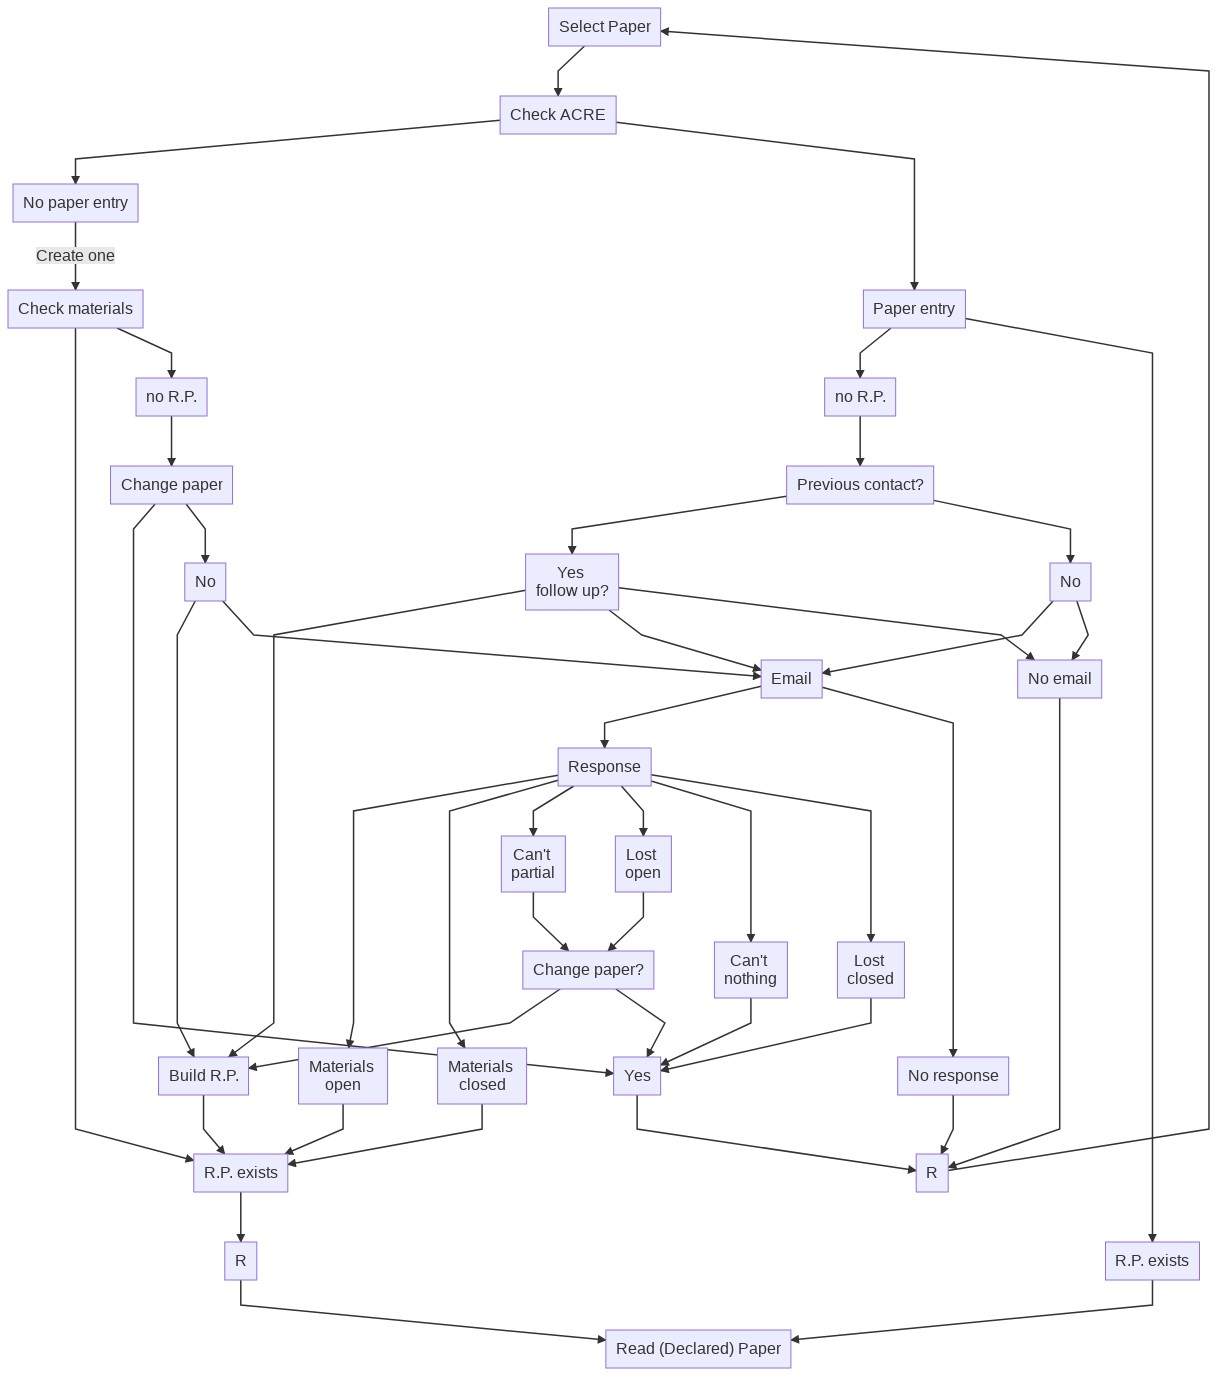
\includegraphics{candidate-paper.jpeg}

\hypertarget{read-sum}{%
\section{Read and summarize the paper.}\label{read-sum}}

Depending on how much time you have, we recommend that you write a short summary of the paper. This will help remind you of the key elements to focus on for the reproduction, and to demonstrate your understanding of the paper (for yourself and potentially for the original author).

When reading/summarizing the paper, you should try to answer the following main questions:

\begin{itemize}
\tightlist
\item
  Would you classify the paper's scientific claims as mainly focused on estimating a causal relationship, estimating/predicting a descriptive statistic of a population, or something else?
\item
  How many scientific claims (descriptive or causal) are investigated in the paper?
\item
  What is the population for which the estimates apply?
\item
  What is the main population that is the focus of the paper as a whole?
\item
  What are the main data sources used in the paper?
\item
  How many outputs are in the paper (tables, figures and inline results)?\\
\item
  What is the main statistical or econometric method used to examine each claim?
\item
  What is the author's preferred specification (or yours if authors are not clear)?
\item
  What are some robustness checks to the preferred specification?
\end{itemize}

\hypertarget{declare-estimates}{%
\section{Declare scope of the exercise.}\label{declare-estimates}}

By now you should have selected a paper that contains a reproduction package, and have a fairly good understanding of the content of the paper. You need not, however, have spent any time reviewing the reproduction package in detail.

At this point, you should clearly specify which part of the paper will be the main focus of your reproduction excercise\footnote{Later in the assessment stage you will be asked to identify all the outputs that are part of your assessment.}. You are asked to focus on specific estimates, represented by a unique combination of claim-output-specification, that represented the authors' preferred specification for a given claim (or yours). If you are planning to scope more than one claim, we strongly advise to start with one and record your results. Then you can initiate another record in ACRE for the second ( third, or more) claim to reproduce, and use the materials and knowledge you developed in the first exercise.

\hypertarget{declare-specific-main-estimates-to-reproduce.}{%
\subsection*{Declare specific main estimates to reproduce.}\label{declare-specific-main-estimates-to-reproduce.}}
\addcontentsline{toc}{subsection}{Declare specific main estimates to reproduce.}

Identify one of the scientific claims, and their corresponding preferred specification, and recorded its magnitude, standard error, and location in the paper (page, table \#, and row and column in the table). If the authors did not explicitly choose a particular estimate, you will be asked to select one. In addition to the preferred estimate, you will be asked to reproduce up to five estimates that correspond to alternative specifications of the preferred estimate.

\hypertarget{declare-possible-robustness-checks-to-main-estimates-optional.}{%
\subsection*{Declare possible robustness checks to main estimates (optional).}\label{declare-possible-robustness-checks-to-main-estimates-optional.}}
\addcontentsline{toc}{subsection}{Declare possible robustness checks to main estimates (optional).}

After reading the paper you might have wonder why the authors did not conduct a specific robustness test. If you think that such analysis could have been done \emph{within the same methodology}, and \emph{using the same data} (eg., including/excluding a subset of the data like ``high-school dropouts'' o ``women''), please specify a robustness test that you would like to test before starting the assessment stage.

This concludes all the elements that you will need to conduct the scoping stage. \textbf{You now have all the elements necesary to complete \href{https://berkeley.qualtrics.com/jfe/form/SV_3UWe5xu3qjeh0c5}{Survey 1}}.

\begin{center}\rule{0.5\linewidth}{0.5pt}\end{center}

\hypertarget{bonus-identify-your-relevant-timeline.}{%
\subsection*{Bonus: Identify your relevant timeline.}\label{bonus-identify-your-relevant-timeline.}}
\addcontentsline{toc}{subsection}{Bonus: Identify your relevant timeline.}

Before you begin working on the three main stages of the reproduction exercise (assessment, improvement, and robustness), it is important to manage expectations (yours and those of your Instructor/Advisor). Be mindful of your time limitations when defining the scope of your reproduction activity. This will be given by the type of exercise chosen by the instructor/academic advisory. These will vary from a short format of a homework over a couple of weeks, to a medium format corresponding to a longer class project that that may take a month to complete, long format of a semester-long project (for example as an undergraduate thesis).

Table 1 shows tentative distribution of time across three different reproduction formats. The scoping and assessment stages are expected to last roughly the same across all formats (with some additional day for the semester long format, foreseeing less experience with research if the reproducer is an undergraduate). Difference emerge in distribution the time for the last two main stages: Improvements and Robustness. For exercises of short duration, we recommend to stay away from any possible improvements to the raw data (or cleaning code), this will intern limit the amount of robustness check (for example by not being able to reconstruct variable according to slightly different definitions), but it should leave plenty of space for testing different specifications at the analysis level.

2 weeks (\textasciitilde{}10 days)

1 month (\textasciitilde{}20 days)

1 semester (\textasciitilde{}100 days)

analysis data

raw data

analysis data

raw data

analysis data

raw data

Scoping

10\% (1 day)

5\% (1 day)

3\% (3 days)

Assessment

25\%

15\%

7\%

Improvement

20\%

0\%

40\%

20\%

30\%

Robustness

30\%

10\%

30\%

30\%

Extension

5\%

0\%

10\%

10\%

\href{https://osf.io/4jvq2/download}{Paper on PBR}. \href{https://dataverse.harvard.edu/dataset.xhtml?persistentId=doi:10.7910/DVN/FPNITS}{Repro package}

\hypertarget{assessment}{%
\chapter{Assessment}\label{assessment}}

The goal of this stage is to conduct a standardized assessment of your chosen paper's computational reproducibility. This stage is designed to record as much of the learning process behind a reproduction as possible. Such a record facilitates future incremental improvements, allowing new reproducers to pick up where others have left off.

First, you will provide a detailed description of the reproduction package. Second, you will connect the outputs you've chosen to reproduce with their corresponding inputs. With these elements in place, you can score the level of reproducibility of each output, and report on paper-level dimensions of reproducibility.

\textbf{Use \href{https://berkeley.qualtrics.com/jfe/form/SV_2gd9Y3XVtjLpZL7}{Survey 2} to record your work as part of this step.}

\emph{Tip:} We recommend that you first focus on one specific output (e.g. ``Table 1''). After completing the assessment for this output, you will have a much easier time translating improvements to other outputs.

\hypertarget{describe-inputs}{%
\section{Describe the inputs.}\label{describe-inputs}}

This section explains how to list all the input materials found or referred to in the reproduction package. First, you'll identify data sources and connect them with their raw data files (when available). Second, you'll locate and provide a brief description of the analytic data files. Finally, you'll locate, inspect, and describe the analytic code used in the paper.

The following terms will be used in this section:

\begin{itemize}
\item
  \textbf{Cleaning code:} A script associated primarily with data cleaning. Most of its content is dedicated to actions such as deleting variables or observations, merging data sets, removing outliers, or reshaping the structure of the data (from long to wide or vice versa).
\item
  \textbf{Analysis code:} A script associated primarily with analysis. Most of its content is dedicated to actions such as running regressions, running hypothesis tests, computing standard errors, and imputing missing values.
\end{itemize}

\hypertarget{describe-the-data-sources-and-raw-data.}{%
\subsection{Describe the data sources and raw data.}\label{describe-the-data-sources-and-raw-data.}}

In the paper to be reproduced, find references to all \emph{data sources} used in the analysis. A data source is usually described in narrative form. For example, if the body of the paper uses text like ``\ldots{}for earnings in 2018 we use the Current Population Survey\ldots{}'', the data source is ``Current Population Survey 2018''. If it is mentioned for the first time on page 1 of the Appendix, its location should be recorded as ``A1''. Do this for all data sources mentioned in the paper.

Data sources also vary by unit of analysis, with some sources matching the same unit of analysis used in the paper (as in previous examples), while others are less clear (e.g., ``our information on regional minimum wages comes from the Bureau of Labor Statistics.'' This should be recorded as ``regional minimum wages from the Bureau of Labor Statistics''.).

Next look at the reproduction package and map the \emph{data sources} mentioned in the paper to the \emph{data files} in the available materials. Record their folder locations relative to the main reproduction folder\footnote{relative location takes the form \texttt{/folder\_in\_rep\_materials/sub\_folder/file.txt}, in contrast to an absolute location that has the form \texttt{username/documents/projects/repros/folder\_in\_rep\_materials/sub\_folder/file.txt}}. In addition to looking at the existing data files, we recommend you review the first lines of all code files (especially cleaning code), looking for lines that call the data sets. Inspecting these scripts may help you understand how different data sources are used, and possibly identify any files missing from the reproduction package.

Record this information in a \href{https://docs.google.com/spreadsheets/d/1LUIdVFH0OfR70C7z07TYeE-uWzKI_JIeWUMaYhqEKK0/edit\#gid=0\&range=A1}{standardized spreadsheet} with the following structure:

\begin{verbatim}
  Raw data information:
      |----------------------|------|-----------------------------------------------|---------------------|---------------------|
      | data_source          | page | data_files                                    | known_missing       | directory           |
      |----------------------|------|-----------------------------------------------|---------------------|---------------------|
      | "Current Population  | A1    | cepr_march_2018.dta                          |                     | \data\              |
      | Survey 2018"         |      |                                               |                     |                     |
      |----------------------|------|-----------------------------------------------|---------------------|---------------------|
      | "DHS 2010 - 2013"    | 4    | nicaraguaDHS_2010.csv;                        | boliviaDHS_2011.csv | \rawdata\DHS\       |
      |                      |      | boliviaDHS_2010.csv; nicaraguaDHS_2011.csv;   |                     |                     |
      |                      |      | nicaraguaDHS_2012.csv; boliviaDHS_2012.csv;   |                     |                     |
      |                      |      | nicaraguaDHS_2013.csv; boliviaDHS_2013.csv    |                     |                     |
      |----------------------|------|-----------------------------------------------|---------------------|---------------------|
      | "2017 SAT scores"    | 4    | Not available                                 |                     | \data\to_clean\     |
      |----------------------|------|-----------------------------------------------|---------------------|---------------------|
      | ...                  | ...  | ...                                           | ...                 | ...                 |
      |----------------------|------|-----------------------------------------------|---------------------|---------------------|
\end{verbatim}

\hypertarget{describe-the-analytic-data-sets.}{%
\subsection{Describe the analytic data sets.}\label{describe-the-analytic-data-sets.}}

List all the analytic files you can find in the reproduction package, and identify their locations relative to the main reproduction folder. Record this information in a \href{https://docs.google.com/spreadsheets/d/1LUIdVFH0OfR70C7z07TYeE-uWzKI_JIeWUMaYhqEKK0/edit\#gid=1299317837\&range=A1}{standardized spreadsheet}.

As you progress through the exercise, add to the spreadsheet a one-line description of each file's main content (for example: \texttt{all\_waves.csv} has the simple description \texttt{data\ for\ region-level\ analysis}). This may be difficult in an initial review, but will become easier as you go along.

The resulting report will have the following structure:

\begin{verbatim}
  Analysis data information:
      |----------------|-----------------------|--------------------------------|
      | analysis_data  | location              | description                    |
      |----------------|-----------------------|--------------------------------|
      | final_data.csv | /analysis/fig1/       | data for figure1               |
      |----------------|-----------------------|--------------------------------|
      | all_waves.csv  | /final_data/v1_april/ | data for region-level analysis |
      |----------------|-----------------------|--------------------------------|
      | ...            | ...                   | ...                            |
      |----------------|-----------------------|--------------------------------|
\end{verbatim}

\hypertarget{desc-scripts}{%
\subsection{Describe the code scripts.}\label{desc-scripts}}

List all code files that you find in the reproduction package and identify their locations relative to the master reproduction folder. Review the beginning and end of each code file and identify the inputs required to successfully run the file. Inputs may include data sets or other code scripts that are typically found at the beginning of the script (e.g., \texttt{load}, \texttt{read}, \texttt{source}, \texttt{run}, \texttt{do} ). For each code file, record all inputs together and separate each item with ``;''. Outputs may include other data sets, figures, or plain text files that are typically at the end of a script (e.g., \texttt{save}, \texttt{write}, \texttt{export}). For each code file, record all outputs together and separate each item with ``;''. Provide a one-line description of what each code file does. Record all this information in the \href{https://docs.google.com/spreadsheets/d/1LUIdVFH0OfR70C7z07TYeE-uWzKI_JIeWUMaYhqEKK0/edit\#gid=1617799822\&range=A1}{standardized spreadsheet} with the following structure:

\begin{verbatim}
  |-------------------|------------------|---------------------|---------------------|----------------------|--------------|
      | file_name         | location         | inputs              | outputs             | description          | primary_type |
      |-------------------|------------------|---------------------|---------------------|----------------------|--------------|
      | output_table1.do  | /code/analysis/  | analysis_data01.csv | output1_part1.txt   | produces first part  | analysis     |
      |                   |                  |                     |                     | of table 1           |              |
      |                   |                  |                     |                     | (unformatted)        |              |
      |-------------------|------------------|---------------------|---------------------|----------------------|--------------|
      | data_cleaning02.R | /code/cleaninig/ | admin_01raw.csv     | analysis_data02.csv | removes outliers     | cleaning     |
      |                   |                  |                     |                     | and missing vals     |              |
      |                   |                  |                     |                     | from raw admin data  |              |
      |-------------------|------------------|---------------------|---------------------|----------------------|--------------|
      | ...               | ...              | ...                 | ...                 | ...                  | ...          |
      |-------------------|------------------|---------------------|---------------------|----------------------|--------------|
\end{verbatim}

As you gain an understanding of each code script, you will likely find more inputs and outputs -- we encourage you to update the \href{https://docs.google.com/spreadsheets/d/1LUIdVFH0OfR70C7z07TYeE-uWzKI_JIeWUMaYhqEKK0/edit\#gid=1617799822\&range=A1}{standardized spreadsheet}. Once finished with the reproduction exercise, classify each code file as \emph{analysis} or \emph{cleaning}. This subjective assessment should be made based on your interpretation of each script's main role.

\hypertarget{diagram}{%
\section{Connect each output to all its inputs}\label{diagram}}

With all the information collected above, you can trace your output to reprodue to its primary sources. Upload the standarized table you build to the decribe the code above into the \href{ADD\%20LINK}{ACRE workflow diagram builder}.

\hypertarget{complete-workflow-information}{%
\subsection{Complete workflow information}\label{complete-workflow-information}}

If you were able to identify all the relevant components in the previous section, the ACRE builder will produce and diagram like the following.

\begin{verbatim}
  table 1
        └───[code] formatting_table1.R
            ├───output1_part1.txt  
            |   └───[code] output_table1.do           
            |       └───[data] analysis_data01.csv
            |          └───[code] data_cleaning01.R
            |             └───[data] survey_01raw.csv
            └───output1_part2.txt  
                └───[code] output_table2.do           
                    └───[data] analysis_data02.csv
                       └───[code] data_cleaning02.R
                          └───[data] admin_01raw.csv  
\end{verbatim}

The ACRE diagram builder will also generate a table that reprents the diagram above in a data set with the following structure:

\begin{verbatim}
  Data representation of diagram behind Table 1.
      |--------|-------|-------------------|---------------------|------------|
      | ouput  | order | component         | depends_on          | inpt_type  |
      |--------|-------|-------------------|---------------------|------------|
      | table1 | 1     | table1            | formatting_table1.R | code       |
      |--------|-------|-------------------|---------------------|------------|
      | table1 | 2     |formatting_table1.R| output1_part2.txt   | output     |
      |--------|-------|-------------------|---------------------|------------|
      | table1 | 3     |formatting_table1.R| output1_part1.txt   | output     |
      |--------|-------|-------------------|---------------------|------------|
      | table1 | 4     | output_table1.do  | analysis_data01.csv | data       |
      |--------|-------|-------------------|---------------------|------------|
      | ...    | ...   | ...               | ...                 | ...        |
      |--------|-------|-------------------|---------------------|------------|
\end{verbatim}

\hypertarget{incomplete-workflow-information}{%
\subsection{Incomplete workflow information}\label{incomplete-workflow-information}}

If there are some components missing, then\ldots{}

{[}Joel and Fernando need to workshop a better solution, until then\ldots{}{]}

Draw diagrams connecting outputs to raw data sources. To do this, find the code script that generates the target output (formatted or not), then find all inputs required to execute the script (including data and other code files). Repeat until you reach the raw data or the last available file.

When a connection cannot be drawn due to a missing component, use the ``-\textbar{}\textbar{}-'' symbol. For more examples of diagrams connecting final output to initial raw data, \protect\hyperlink{additional-diagrams}{see here}.\\
This diagram can be represented in data format by specifying how each component depends on its inputs. For example:

Record this information in the \href{https://docs.google.com/spreadsheets/d/1LUIdVFH0OfR70C7z07TYeE-uWzKI_JIeWUMaYhqEKK0/edit\#gid=1384504774\&range=A1}{standardized spreadsheet}.
If you have difficulty translating the diagram into a spreadsheet, you can draw it with pen and paper, take a picture and upload it to the assessment survey.

\hypertarget{score}{%
\section{Assign a reproducibility score.}\label{score}}

Once all possible inputs have been identified, and there is a clear understanding of the connection between the outputs and inputs, you can start to assess the output-specific level of reproducibility.

The following concepts will be used in this section:

\begin{itemize}
\item
  \textbf{Computationally Reproducible from Analytic data (CRA):} The output can be reproduced with minimal effort starting from the analytic data sets.
\item
  \textbf{Computationally Reproducible from Raw data (CRR):} The output can be reproduced with minimal effort from the raw data sets.
\item
  \textbf{Minimal effort:} One hour or less are required to run the code, not including computing time.
\end{itemize}

\hypertarget{levels-of-computational-reproducibility-for-a-specific-output}{%
\subsection{Levels of Computational Reproducibility for a Specific Output}\label{levels-of-computational-reproducibility-for-a-specific-output}}

Here we outline different levels of computational reproducibility. Each level is defined by availability of data and materials, and whether or not some type of reproducibility is achieved. In addition, for each level we briefly describe the type of improvements that can be done to improve the current reproducibility. In the next chapter we'll describe each possible improvement in more detail.

The assessment is made at the output level -- a paper can be highly reproducible for its main results, but suffer from low reproducibility for other outputs. The assessment is made using a 10-point scale, where 0 represents that, under current circumstances, reproducers cannot access any reproduction package, while 10 represents access to all the materials and that the target outcome can be reproduced starting from raw data.

\begin{itemize}
\item
  \textbf{Level 1 (L1):} No data or code are available. Possible improvements include adding: raw data (+AD), analysis data (+RD), cleaning code (+CC), and analysis code (+AC).
\item
  \textbf{Level 2 (L2):} Code scripts are available, but no data are available. Possible improvements include adding: raw data (+AD) and analysis data (+RD).
\item
  \textbf{Level 3 (L3):} Analytic data are available, but raw data and code are not. Possible improvements include adding: raw data (+RD) and analysis code (+AC).
\item
  \textbf{Level 4 (L4):} Analytic data sets and analysis code are available. However, code does not run or produces different results than those in the paper (not CRA). Possible improvements include obtaining raw data (+RD) or debugging the analysis code (DAC).
\item
  \textbf{Level 5 (L5):} Analytic data sets and analysis code are available. They produce the same results as presented in the paper (CRA). The reproducibility package may be improved by obtaining the original raw data sets, or by documenting the steps required to obtain those files.
\item
  \textbf{Level 6 (L6):} Analytic data and raw data are available. However, some or all cleaning and analysis code are missing. Possible improvements include: adding analysis code (+AC) and/or cleaning code (+CC).
\item
  \textbf{Level 7 (L7):} All data and analysis code are available. However, the code does not run or produces different results than those presented in the paper (not CRA). Possible improvements include: adding the missing cleaning code (+CD) or debugging the analysis code (DAC).
\item
  \textbf{Level 8 (L8):} All data and analysis code are available, but cleaning code may be missing. They produce the same results as presented in the paper (CRA). The reproducibility package may be improved by adding the missing cleaning code (+CD).
\item
  \textbf{Level 9 (L9):} All materials (raw data, analytic data, cleaning code, and analysis code) are available. However, the code does not run or produces different results than those presented in the paper (not CRR and not CRA). Possible improvements include: debugging the cleaning code (DCC) or debugging the analysis code (DAC).
\item
  \textbf{Level 10 (L10):} All materials (raw data, analytic data, cleaning code, and analysis code) are available. The analysis code produces the same output as presented in the paper (CRA). However, the cleaning code does not run or produces different results that those presented in the paper (not CRR). Possible improvements include: debugging the cleaning code (DCC).
\item
  \textbf{Level 11 (L11):} All materials are available and produce the same results as presented in the paper with minimal effort, starting from the analytic data (yes CRA) or the raw data (yes CRR).
\end{itemize}

The following figure summarizes the different levels of computational reproducibility (for any given output). For each level, there will be improvements that: have been made (-), can be made to move up one level of reproducibility (\texttt{✔}), or are out of reach given the current level of reproducibility (\texttt{x}).

\begin{verbatim}
                Figure 1: Levels of Computational Reproducibility    

                                 | Availavility of materials, and reproducibility |
                                 |------------------------------------------------|
                                 |Analysis| Analysis| CRA | Cleaning| Raw   | CRR |
                                 |Code    | Data    |     | Code    | Data  |     |
                                 ---------|---------|-----|---------|-------|-----|
                                 | P | C  | P  | C  |     | P  |  C | P | C |     |
L1: No materials.................| -   -  | -    -  |  -  |  -    - | -   - |  -  |     
L2: Only code and/or docs........| ✔   ✔  | -    -  |  -  |  -    - | -   - |  -  |     
L3: Partial analyiss data & code.| ✔   ✔  | ✔    -  |  -  |  -    - | -   - |  -  |
L4: All analysis data & code.....| ✔   ✔  | ✔    ✔  |  -  |  -    - | -   - |  -  |
L5: Reproducible from analysis...| ✔   ✔  | ✔    ✔  |  ✔  |  -    - | -   - |  -  |
L6: Some cleaning code...........| ✔   ✔  | ✔    ✔  |  ✔  |  ✔    - | -   - |  -  |
L7: All cleaning code............| ✔   ✔  | ✔    ✔  |  ✔  |  ✔    ✔ | -   - |  -  |
L8: Some raw data................| ✔   ✔  | ✔    ✔  |  ✔  |  ✔    ✔ | ✔   - |  -  |
L9: All raw data.................| ✔   ✔  | ✔    ✔  |  ✔  |  ✔    ✔ | ✔   ✔ |  -  |
L10:Reproducible from raw data...| ✔   ✔  | ✔    ✔  |  ✔  |  ✔    ✔ | ✔   ✔ |  ✔  |
\end{verbatim}

Choose the appropriate level of computational reproducibility and record it using the following format.

\begin{verbatim}
  |-------------|-------|------------------------|------------|
      | output_name | level | additional_explanation | other_info |
      |-------------|-------|------------------------|------------|
      | table 1     | 4     |                        | ...        |
      |-------------|-------|------------------------|------------|
      | table 2     | 7     |                        | ...        |
      |-------------|-------|------------------------|------------|
      | figure 1    | 5     |                        | ...        |
      |-------------|-------|------------------------|------------|
      | ...         | ...   | ...                    | ...        |
      |-------------|-------|------------------------|------------|
\end{verbatim}

Record this information in the \href{https://docs.google.com/spreadsheets/d/1LUIdVFH0OfR70C7z07TYeE-uWzKI_JIeWUMaYhqEKK0/edit\#gid=1384504774\&range=A1}{standarized spreadsheet}. You will be asked to provide this information in the \href{ADD\%20LINK}{assessment and improvement survey}.

To present each category above as levels that reflect a gradient of improvement, we need to make explicit the following underlying valuations.

\begin{itemize}
\tightlist
\item
  L1: The worst is to have no access to any data or code.\\
\item
  L2: Having only some code is better than nothing, but worst than any data.
\item
  L3: Having analytic data but not code is better than having code and no data.
\item
  L4 and L5: Conditional on having all analytic material. Reproducible is better than not
\item
  L6: Having raw and analytic data, even without any code, is better than having CRA.\\
\item
  L7: Given that there is raw and analysis data, having a cleaning code only does not add much. having analysis code does add (to lvl 7 and lvl 8 if CRA)\\
\item
  L9: Having all materials that but not being able to reproduce is better than all previous cases. Achieving CRA (lvl 10) and CRR (lvl 11) are the best levels according to these criteria.
\end{itemize}

The reproducer and/or reader of this information can disagree with this subjective valuations. In this scenario, the levels should be understood as unordered categories, or ordered under different criteria. The reader of these guidelines are also encouraged to submit suggested edits using the ADD IMAGE button above.

\hypertarget{reproducibility-dimensions-at-the-paper-level}{%
\subsection{Reproducibility dimensions at the paper level}\label{reproducibility-dimensions-at-the-paper-level}}

In addition to an output-specific assessment of computational reproducibility, several practices can facilitate a paper's overall computational reproducibility. These practices are described in detail in the Improvement chapter. In the Assessment section, it is only required that you verify whether the original reproduction package made use of any of the following:

\begin{itemize}
\tightlist
\item
  master script that runs all steps
\item
  readme file
\item
  standard file organization\\
\item
  version control
\item
  analysis uses open source software\\
\item
  dynamic document\\
\item
  computing capsule (e.g.~CodeOcean, Binder, etc.)
\end{itemize}

Congratulations! You have now completed the Assessment stage. You have provided a concrete building block of knowledge to improve understanding of the state of reproducibility in Economics.

Please continue to the \protect\hyperlink{improvements}{next section} where you can help to improve it!

\hypertarget{improvements}{%
\chapter{Improvements}\label{improvements}}

After completing an assessment of the paper's reproducibility packages, you can start proposing ways to improve it's reproducibility. Making improvements provides an opportunity to gain deeper understanding of the paper's methods, findings, and overall contribution. Each contribution can also be assessed and used by the wider ACRE community--other students and researchers using the ACRE platform around the world.

As in the Assessment section, we recommend that you first focus on one specific output (e.g., ``Table 1''). After making improvements to this first output, you will have a much easier time translating those improvements to other outputs.

\textbf{Use Survey 2 to record your work as part of this step.}

\hypertarget{types-of-output-level-improvements}{%
\section{Types of output-level improvements}\label{types-of-output-level-improvements}}

\hypertarget{rd}{%
\subsection{Adding missing raw data files or meta-data (+RD)}\label{rd}}

Reproduction packages often do not include all original \protect\hyperlink{describe-inputs}{raw datasets}. To obtain any missing raw data, or information about them, follow these steps:

\begin{enumerate}
\def\labelenumi{\arabic{enumi}.}
\tightlist
\item
  Identify a specific missing file. During \protect\hyperlink{assessment}{Assessment}, you identified all data sources from the paper's body and appendices (column \texttt{data\_source} in \href{https://docs.google.com/spreadsheets/d/1LUIdVFH0OfR70C7z07TYeE-uWzKI_JIeWUMaYhqEKK0/edit\#gid=0\&range=A1}{this standarized spreadsheet}). However, some data sources (as collected by the original investigators) might be missing one or more data files. You can sometimes find the specific name of those files by looking at the beginning of the cleaning code scripts. If you find the name of the file, record it in the \texttt{data\_file} field of the \href{https://docs.google.com/spreadsheets/d/1LUIdVFH0OfR70C7z07TYeE-uWzKI_JIeWUMaYhqEKK0/edit\#gid=0\&range=A1}{same spreadsheet} as above. If not, recorded it as ``Some (or all) of the files used in the paper corresponding to data source X''.\\
\item
  Verify whether this file (or files) can be easily obtained from the web.

  \begin{itemize}
  \tightlist
  \item
    2.1 - If yes: obtain the missing files and add them to the reproduction package. Make sure to obtain permission from the origina author to repost this data. See \protect\hyperlink{tips-for-communication}{tips for communication} for a template email.\\
  \item
    2.2 - If no: proceed to step 3.\\
  \end{itemize}
\item
  \href{ADD\%20LINK}{Use the ACRE database} to verify whether there have been previous attempts to contact the authors regarding this paper.\\
\item
  Contact the original authors and politely request the original materials. Be mindful of the authors' time, and remember that the paper you are trying to reproduce was possibly published at a time when standards for computational reproducibility were different. See \protect\hyperlink{tips-for-communication}{tips for communication} for sample language on how to approach authors.\\
\item
  If the data sets are not available due to confidentiality or proprietary issues, you can still improve the reproduction package by providing detailed instructions for future researchers to follow, including contact information and possible costs.
\end{enumerate}

In addition to trying to obtain raw data, you can also contribute by obtaining missing analytic data.

\hypertarget{ad}{%
\subsection{Adding missing analytic data files (+AD)}\label{ad}}

\protect\hyperlink{describe-inputs}{Analytic data} can be missing for two reasons: (i) raw data exists, but the procedures to transform it into analytic data are not fully reproducible, or (ii) some or all raw data is missing and some or all analytic data is not included in the original reproduction package. To obtain any missing analytic data, follow these steps:

\begin{enumerate}
\def\labelenumi{\arabic{enumi}.}
\tightlist
\item
  Identify the specific name of the missing data set. Typically this information can be found in some of the analysis code that calls the data to perform an analysis (eg \texttt{analysis\_data\_03.csv}).\\
\item
  Verify that the data cannot be obtained by running the data cleaning code over the raw data.\\
\item
  \href{ADD\%20LINK}{Use the ACRE database} to verify if previous attempts have been made to contact the authors about this data.\\
\item
  \protect\hyperlink{tips-for-communication}{Contact the authors} and request the specific data set.
\end{enumerate}

\hypertarget{ac}{%
\subsection{Adding missing analysis code (+AC)}\label{ac}}

\protect\hyperlink{describe-inputs}{Analysis code} can be added when analytic data files are available, but some or all methodological steps are missing from the code. In this case, follow these steps:

\begin{enumerate}
\def\labelenumi{\arabic{enumi}.}
\item
  Identify the specific line or paragraph in the paper that describes the analytic step that is missing from the code (e.g., ``We impute missing values to\ldots{}'' or ``We estimate this regression using a bandwidth of\ldots{}'').
\item
  Identify the code file and the approximate line in the script where the analysis can be carried out. If no relevant code file is found, identify the location of the missing file relative to the steps in the \protect\hyperlink{diagram}{reproduction diagram}.
\item
  \href{ADD\%20LINK}{Use the ACRE database} to verify if previous attempts have been made to contact the authors about this issue.
\item
  \protect\hyperlink{tips-for-communication}{Contact the authors} and request the specific code files.
\item
  If the authors don't respond, we encourage you to attempt to recreate the analysis using your own interpretation of the paper, and making explicit your assumptions when filling in any gaps.
\end{enumerate}

\hypertarget{cc}{%
\subsection{Adding missing data cleaning code (+CC)}\label{cc}}

\protect\hyperlink{describe-inputs}{Data cleaning (processing)} code might be added when steps are missing in the creation or re-coding of variables, merging, subsetting of the data sets, or other steps related to data cleaning and processing. You should follow the same steps you used when adding missing analysis code (1-5).

\hypertarget{dac}{%
\subsection{Debugging analysis code (DAC)}\label{dac}}

Whenever code is available in the reproduction package, you should be able to debug those scripts. There are four types of debugging that can improve the reproduction package:

\begin{itemize}
\tightlist
\item
  \emph{Code cleaning:} Simplify the instructions (e.g., by wrapping repetitive steps in a function or a loop) or remove redundant code (i.e., old code that was commented out) while keeping the original output intact.

  \begin{itemize}
  \tightlist
  \item
    \emph{Performance improvement:} Replace instructions with new ones that perform the same tasks but take less time (e.g., choose one numerical optimization algorithm over another, but obtain the same results).\\
  \item
    \emph{Environment set up:} Modify the code to include correct paths to files, specific versions of software, and instructions to install missing packages or libraries.\\
  \item
    \emph{Correcting errors:} A coding error will occur when a section of the code in the reproduction package executes a procedure that is in direct contradiction with the intended procedure expressed in the documentation (i.e., paper or code comments). For example, an error will happen if the paper specifies that the analysis is performed on a population of males, but the code restricts the analysis to females only. Please follow the \href{ADD\%20LINK}{ACRE procedure to report coding errors}.
  \end{itemize}
\end{itemize}

\hypertarget{debugging-cleaning-code-dcc}{%
\subsection{Debugging cleaning code (DCC)}\label{debugging-cleaning-code-dcc}}

Use the same steps as you took to debug the analysis code, but report them separately.

\hypertarget{reporting-results}{%
\subsection{Reporting results}\label{reporting-results}}

Track all the different types of improvements you make and record in \href{https://docs.google.com/spreadsheets/d/1LUIdVFH0OfR70C7z07TYeE-uWzKI_JIeWUMaYhqEKK0/edit\#gid=0\&range=A3}{this standarized spreadsheet} with the following structure:

\begin{verbatim}
   Level-specific quality improvements: add data/code, debug code.

       | output_name | imprv | description_of_added_files        | lvl |
       |-------------|-------|-----------------------------------|-----|
       | table 1     | +AD   |        ADD EXAMPLES               |  5  |
       | table 1     | +RD   |        ADD EXAMPLES               |  5  |
       | table 1     | DCC   |        ADD EXAMPLES               |  5  |
       | figure 1    | +CC   |                                   |  6  |
       | figure 1    | DAC   |                                   |  6  |
       | inline 1    | DAC   |                                   |  8  |
       | ...         | ...   | ...                               | ... |  
\end{verbatim}

\hypertarget{paper-level}{%
\section{Types of paper-level improvements}\label{paper-level}}

There are at least six additional improvements you can make to improve a paper's overall reproducibility. These additional improvements can be applied across all reproducibility levels (including level 10).

\begin{enumerate}
\def\labelenumi{\arabic{enumi}.}
\tightlist
\item
  Set up the reproduction package using version control software, such as Git.
\item
  Improve documentation by adding extensive comments to the code.
\item
  Integrate the documentation with code by adapting the paper into a literate programming environment (e.g., using Jupyter notebooks, RMarkdown, or a Stata Dynamic Doc).
\item
  If the code was written using a proprietary statistical software (e.g., Stata or Matlab), re-write it using an open source statistical software (e.g., R, Python, or Julia).
\item
  Re re-organize the reproduction package into a set of folders and sub-folders that follow \href{https://www.projecttier.org/tier-protocol/specifications/\#overview-of-the-documentation}{standardized best practices}, and add a master script that executes all the code in order, with no further modifications. \href{https://github.com/AEADataEditor/replication-template}{See AEA's reproduction template}.\\
\item
  Set up a computing capsule that executes the entire reproduction in a web browser without needing to install any software. For examples, see \href{https://mybinder.org/}{Binder} and \href{https://codeocean.com/}{Code Ocean}.
\end{enumerate}

\hypertarget{reporting-improvements}{%
\subsection{Reporting improvements}\label{reporting-improvements}}

You will be asked to provide this information in the \href{ADD\%20LINK}{Assessment and Improvement Survey}.

\hypertarget{robust}{%
\chapter{Checking for Robustness}\label{robust}}

{[}UNDER CONSTRUCION{]}

\begin{itemize}
\tightlist
\item
  Identify all possible analytical choices: original and repeated ones.\\
\item
  Identify type of choice.\\
\item
  Identify choice value.
\item
  Suggest choice alternative and justify (one line)
\end{itemize}

\hypertarget{id-analy}{%
\section{Identifying Analytical Choices}\label{id-analy}}

As part of the requirements to \href{requirements_comprehension.md}{demonstrate comprehension of the paper and the code} researchers conducting the reproduction will be asked to record all the analytical choices identified during the code review process. This is done in two steps: first adding comment lines into the code files where an analytic choice are found, and second, compiling those analytic choices into a standardized data set.

In your copy of the replication code, add the comment \texttt{“\#\ ANALYTICAL\ CHOICE\ OF\ TYPE\ \_\_\_\_.\ RECORDED\ FOR\ THE\ FIRST\ TIME\ {[}HERE\ or\ IN\ "FILE\_NAME-LINE\_NUMBER"{]}”} above each analytical choice detected in the code. Possible types of analytical choices include (but are not limited to):

\begin{itemize}
\tightlist
\item
  Analytical choices in data cleaning code:

  \begin{itemize}
  \tightlist
  \item
    Variable definition\\
  \item
    Data sub-setting\\
  \item
    Data reshaping (merge, append, long/gather, wide/spread)\\
  \item
    Others (specify as ``processing - other'')
  \end{itemize}
\item
  Analytical choices in analysis code:

  \begin{itemize}
  \tightlist
  \item
    Regression function (link function)\\
  \item
    Key parameters (tuning, tolerance parameters, etc.)\\
  \item
    Controls\\
  \item
    Adjustment of standard errors\\
  \item
    Choice of weights\\
  \item
    Treatment of missing values\\
  \item
    Imputations
  \item
    Other (specify as ``methods - other'')
  \end{itemize}
\end{itemize}

Once finished, transcribe all the information on analytical choices into a data set. For the \texttt{source} field type ``original'' whenever the analytical choice is identified for the first time, and \texttt{file\_name-line\ number} every time that the same analytical choice is applied subsequently (for example if a analytic choice is identified for the first time in line 103 and for a second in line 122 their respective values for the \texttt{source} field should be \texttt{original} and \texttt{code\_01.do-L103} respectively).

The resulting data base should have the \href{https://docs.google.com/spreadsheets/d/1nZuJSHswbZgaaIfBcyIUGPwG-WIP8zE1Oambud-WoDc/edit?usp=sharing}{following structure}:

\begin{longtable}[]{@{}lllll@{}}
\toprule
\begin{minipage}[b]{0.10\columnwidth}\raggedright
file\_name\strut
\end{minipage} & \begin{minipage}[b]{0.11\columnwidth}\raggedright
line\_number\strut
\end{minipage} & \begin{minipage}[b]{0.18\columnwidth}\raggedright
choice\_type\strut
\end{minipage} & \begin{minipage}[b]{0.28\columnwidth}\raggedright
choice\_value\strut
\end{minipage} & \begin{minipage}[b]{0.18\columnwidth}\raggedright
Source\strut
\end{minipage}\tabularnewline
\midrule
\endhead
\begin{minipage}[t]{0.10\columnwidth}\raggedright
code\_01.do\strut
\end{minipage} & \begin{minipage}[t]{0.11\columnwidth}\raggedright
73\strut
\end{minipage} & \begin{minipage}[t]{0.18\columnwidth}\raggedright
data subsetting\strut
\end{minipage} & \begin{minipage}[t]{0.28\columnwidth}\raggedright
males\strut
\end{minipage} & \begin{minipage}[t]{0.18\columnwidth}\raggedright
original\strut
\end{minipage}\tabularnewline
\begin{minipage}[t]{0.10\columnwidth}\raggedright
code\_01.do\strut
\end{minipage} & \begin{minipage}[t]{0.11\columnwidth}\raggedright
122\strut
\end{minipage} & \begin{minipage}[t]{0.18\columnwidth}\raggedright
variable definition\strut
\end{minipage} & \begin{minipage}[t]{0.28\columnwidth}\raggedright
income = wages + capital gains\strut
\end{minipage} & \begin{minipage}[t]{0.18\columnwidth}\raggedright
``code\_01.do-L103''\strut
\end{minipage}\tabularnewline
\begin{minipage}[t]{0.10\columnwidth}\raggedright
code\_05.R\strut
\end{minipage} & \begin{minipage}[t]{0.11\columnwidth}\raggedright
143\strut
\end{minipage} & \begin{minipage}[t]{0.18\columnwidth}\raggedright
controls\strut
\end{minipage} & \begin{minipage}[t]{0.28\columnwidth}\raggedright
age, income, education\strut
\end{minipage} & \begin{minipage}[t]{0.18\columnwidth}\raggedright
original\strut
\end{minipage}\tabularnewline
\begin{minipage}[t]{0.10\columnwidth}\raggedright
\ldots{}\strut
\end{minipage} & \begin{minipage}[t]{0.11\columnwidth}\raggedright
\ldots{}\strut
\end{minipage} & \begin{minipage}[t]{0.18\columnwidth}\raggedright
\ldots{}\strut
\end{minipage} & \begin{minipage}[t]{0.28\columnwidth}\raggedright
\ldots{}\strut
\end{minipage} & \begin{minipage}[t]{0.18\columnwidth}\raggedright
\ldots{}\strut
\end{minipage}\tabularnewline
\bottomrule
\end{longtable}

\hypertarget{id-analy}{%
\section{Identifying Choice Type}\label{id-analy}}

\hypertarget{id-analy}{%
\section{Identifying Analytical Choices}\label{id-analy}}

\hypertarget{id-val}{%
\section{Identifying Analytical Value}\label{id-val}}

\hypertarget{test-rob}{%
\section{Choose and justify alternative values for analytical choices}\label{test-rob}}

\hypertarget{test-the-robustness-of-results}{%
\section{Test the robustness of results}\label{test-the-robustness-of-results}}

Test the robustness of results to alternative (sensible) specifications

\begin{itemize}
\tightlist
\item
  Identify sensible alternatives to analytical choices.

  \begin{itemize}
  \tightlist
  \item
    Sample from sensible analytical choices and re-run: report how much do results change as fraction of standard deviations.\\
  \item
    Jackknife the preferred estimate.
  \item
    Use ML to select among covariates\ldots{}
  \end{itemize}
\end{itemize}

\hypertarget{concluding-the-reproduction}{%
\chapter{Concluding the reproduction}\label{concluding-the-reproduction}}

{[}UNDER CONSTRUCTION{]} but testing now

Walk the students on checking that they have completed all the steps and where can they see their output.

\hypertarget{final-products}{%
\section{Final products}\label{final-products}}

\begin{itemize}
\item
  One-page introduction describing why you chose this paper
\item
  Two-page summary of paper
\item
  2 Completed surveys:

  \begin{itemize}
  \tightlist
  \item
    i - General information about the paper and specific
    information about output to reproduce.\\
  \item
    ii - Assessment of how (computationally) reproducible is the paper;
    description of improvements to its reproducibility; record of all the
    analytical choices identified in the exercise.
  \end{itemize}
\item
  ACRE report card with all the improvements that were created by the researcher reproducing the paper. The list of improvements will be made public and original authors will receive a copy of the report card. The option of anonymity will be provided to the researchers reproducing the paper.
\item
  New Readme file (autogenerated).
\item
  Data with all analytical choices identified.
\item
  ?? Narrated description of improvements to original CR of the paper, assessment of robustness of results. Lessons from the exercise and possible future extensions.
\end{itemize}

\hypertarget{guidance-for-a-constructive-exchange-between-reproducers-and-original-authors}{%
\chapter{Guidance for a Constructive Exchange Between Reproducers and Original Authors}\label{guidance-for-a-constructive-exchange-between-reproducers-and-original-authors}}

The purpose of this chapter is to facilitate constructive and respectful communication between reproducers (you) and original authors. Exchanges that contain charged or adversarial language can damage professional relationships and hamper scientific progress. Janz and Freese (\href{https://www.mzes.uni-mannheim.de/openscience/wp-content/uploads/2019/01/Janz-Freese_-Good-and-Bad-Replications-1.pdf}{2019}) articulate two important steps reproducers can take to ensure their interactions with original authors are constructive. We provide a summary below and encourage you to follow this guidance. Remember the golden rule of reproductions (and replications): \emph{treat others and their work, as you would like others to treat you and your work!}

\textbf{1. Carefully and transparently plan your study.}

\begin{enumerate}
\def\labelenumi{\alph{enumi}.}
\tightlist
\item
  Clearly state that you are conducting a reproduction of the original work.

  \begin{enumerate}
  \def\labelenumii{\alph{enumii}.}
  \setcounter{enumii}{1}
  \tightlist
  \item
    Explain why you have chosen this study. Try to proactively address potential concerns for selection bias.\\
  \item
    Explain how ``far'' your results must deviate from the original work before claiming that the study could not be reproduced. Engage deeply with the substantive literature to ensure that your interpretation of differences between the original and reproduction is thorough and acceptable to other authors in the field.
  \end{enumerate}

  \textbf{2. Use professional and sensitive language. Discuss potential discrepancies between your work and the original paper just like you would have done for your own work.}

  \begin{enumerate}
  \def\labelenumii{\alph{enumii}.}
  \tightlist
  \item
    Avoid binary judgments and statements like ``failed to reproduce.'' Clearly state which results reproduced and which did not (e.g., ``we successfully reproduced X, but failed to reproduce Y'') unless you uncover apparent scientific misconduct (e.g.~see \href{https://osf.io/qy2se/}{Broockman, Kalla and Aronow, 2015}).\\
  \item
    Talk about \emph{the study, not the author}, to avoid making it personal. Make clear what the positive contribution of the original article is. Consider sending a copy of your reproduction report to the original authors.\\
  \item
    Discuss what your reproduction contributes to the literature, and refrain from claiming to give the final answer to the question.\\
  \item
    For papers published five or more years ago, be mindful that norms for reproducibility have evolved since then.\\
  \item
    Remember, \emph{the goal is not to criticize previous work or hunt for errors, but to move the literature forward!}
  \end{enumerate}
\end{enumerate}

To help put these recommendations into practice, we provide template language for common scenarios that reproducers and authors may encounter in their interactions.

While we hope that you find these useful, note that they are \emph{only recommendations}, and you are welcome to modify them based on the context and needs of your specific project. Feel free to contact us if you need more guidance or would like to provide feedback on these materials.

\hypertarget{for-reproducers-contacting-the-authors-of-the-original-study}{%
\section{For Reproducers Contacting the Authors of the Original Study}\label{for-reproducers-contacting-the-authors-of-the-original-study}}

Consider the following \emph{before} you contact the original author:

\begin{enumerate}
\def\labelenumi{\arabic{enumi}.}
\tightlist
\item
  Carefully read all footnotes, appendices, tables, captions, etc. to learn if, how, and where reproduction materials are provided. Follow this \href{https://social-science-data-editors.github.io/guidance/Verification_guidance.html}{Data and Code Guidance} to determine whether you have everything before you start. A few things to consider:

  \begin{itemize}
  \tightlist
  \item
    A \emph{Readme} file, if available, would be a good place to start. All papers published in AEA journals after July 2019 should have such documentation.\\
  \item
    Check whether there are any restrictions to accessing the data or code, and whether there are instructions on how to access these files for the purpose of reproduction.
  \end{itemize}

  \begin{enumerate}
  \def\labelenumii{\arabic{enumii}.}
  \setcounter{enumii}{1}
  \item
    If reproduction materials are not readily available in the location where the article is published (e.g., the journal website), check the authors' websites, Dataverse profiles, the \href{https://www.icpsr.umich.edu/icpsrweb/}{ICPSR Publications Related Archive}, and other relevant archives and/or data repositories.
  \item
    If steps 1 and 2 don't work, contact the corresponding author (copying the co-authors, if any), consolidating your requests into as few emails as possible. In your email, make sure to include the following details:

    \begin{itemize}
    \tightlist
    \item
      Basic information about the paper being reproduced (include title, version, date, and a DOI link (or just a URL));\\
    \item
      Context for the reproduction (as part of a class exercise, thesis, etc.) and a notice that the outcome will be recorded in the ACRE reproducibility database;\\
    \item
      Items from the reproduction package that are missing, as well as locations where you had (unsuccessfully) searched for them;\\
    \item
      Use plan: Will the materials be used exclusively for this project? Ask for permission to share the data publicly.\\
    \item
      Right to consultation and results: Will you share the outcome of the reproduction exercise with the original authors?\\
    \item
      A deadline to respond (we suggest at least two weeks).
    \end{itemize}
  \item
    Follow up if you don't get a response within two weeks (or whatever deadline you set), and include any details or clarifications that were left out in your first email.
  \end{enumerate}
\end{enumerate}

\hypertarget{contacting-the-original-authors-to-request-a-missing-reproduction-package-or-missing-items}{%
\subsection{Contacting the original author(s) to request a missing reproduction package or missing items}\label{contacting-the-original-authors-to-request-a-missing-reproduction-package-or-missing-items}}

\textbf{Template email:}

\begin{quote}
\textbf{Subject:} Reproduction materials for \texttt{{[}“Title\ of\ the\ paper”{]}}
\end{quote}

\begin{quote}
Dear Dr. \texttt{{[}Lastname\ of\ Corresponding\ Author{]}},

I am contacting you about reproduction materials for your paper titled \texttt{{[}Title{]}} which was published in \texttt{{[}Journal{]}} in \texttt{{[}year{]}} (vol \texttt{{[}volume{]}}, no. \texttt{{[}no.{]}}), \texttt{{[}link{]}}.
I am a \texttt{{[}graduate\ student/postdoc/other\ position{]}} at \texttt{{[}Institution{]}}, and I'm working to reproduce this paper as part of a class exercise. \texttt{{[}Add\ context\ for\ why\ you\ want\ to\ reproduce\ this\ particular\ paper\ using\ neutral\ language\ (e.g.,\ "This\ is\ a\ seminal\ paper\ in\ my\ field"),\ avoiding\ any\ statements\ that\ would\ put\ the\ respondent\ on\ the\ defensive{]}}.

To be able to reproduce the paper in full, I hope that you can share the following items: {[}\texttt{list\ items\ missing\ from\ reproduction\ package,\ preferably\ bulleted\ if\ more\ than\ one\ (raw/analytic\ data,\ code,\ protocols\ for\ conducting\ the\ experiment,\ etc.)}{]}. I have already searched \texttt{{[}locations\ where\ you\ searched\ for\ items,\ with\ links\ provided{]}}, however I was not able to locate the items there. You can be assured that I will not share any of the materials without your permission, and I will use them exclusively for the purpose of this exercise. Let me know if there are any legal or ethical restrictions that apply to all or parts of the reproduction materials so that I can take that into consideration during this exercise.

Note that I will record the outcome of my reproduction on the Advancing Computational Reproducibility in Economics (ACRE) \href{https://www.bitss.org/ecosystem/acre/}{platform}, an online catalog of reproduction projects in economics. ACRE is hosted by the \href{https://www.bitss.org/}{Berkeley Initiative for Transparency in the Social Sciences (BITSS)}. Let me know if you would like me to share the outcome of my exercise with you and whether you are interested in providing a response.

Since I am required to complete this project by \texttt{{[}date{]}}, I would appreciate your response by \texttt{{[}deadline{]}}.

Let me know if you have any questions. Please also feel free to contact my supervisor/instructor \texttt{{[}Name\ (email){]}} for further details on this exercise. Thank you in advance for your help!

Best regards,\\
\texttt{{[}Reproducer{]}}
\end{quote}

\hypertarget{asking-for-additional-guidance-when-some-materials-have-been-shared}{%
\subsection{Asking for additional guidance when some materials have been shared}\label{asking-for-additional-guidance-when-some-materials-have-been-shared}}

\emph{Note:} Even when a corresponding author has shared a reproduction package, you may still run into challenges in interpreting or executing the materials. That shouldn't discourage you from asking the corresponding author to provide clarifications or share missing materials. As in the first scenario described above, demonstrate that you made an honest effort to reproduce the work using the available resources and try to consolidate your requests into as few emails as possible.

\textbf{Template email:}

\begin{quote}
\textbf{Subject:} Clarification for reproduction materials for \texttt{{[}“Title\ of\ the\ paper”{]}}
\end{quote}

\begin{quote}
Dear Dr. \texttt{{[}Lastname\ of\ Corresponding\ Author{]}},

Thank you for sharing the materials. They have been immensely helpful for my work.

Unfortunately, I ran into a few issues as I delved into the reproduction exercise, and I think your guidance would be helpful in resolving them. \texttt{{[}Describe\ the\ issues\ and\ how\ you\ have\ tried\ to\ resolve\ them.\ Describe\ whatever\ files\ or\ parts\ of\ the\ data\ or\ code\ are\ missing.\ Refer\ to\ examples\ 1\ and\ 2\ below\ for\ more\ details{]}}.

Thank you in advance for your help.

Best regards,\\
\texttt{{[}Reproducer{]}}
\end{quote}

\textbf{1: An example of well described issues:}

\begin{quote}
Specifically, I am attempting to reproduce OUTPUT X (e.g., table 1, figure 3). I found that the following components are required to reproduce to reproduce OUTPUT X:
\end{quote}

\begin{verbatim}
 OUTPUT X
        └───[code] formatting_table1.R
            ├───output1_part1.txt  
            |   └───[code] output_table1.do           
            |       └───[data] analysis_data01.csv
            |          └───[code] data_cleaning01.R*
            |             └───[data] UNKNOWN
            └───output1_part2.txt  
                └───[code] output_table2.do           
                    └───[data] analysis_data02.csv
                       └───[code] data_cleaning02.R
                          └───[data] admin_01raw.csv* 
\end{verbatim}

\begin{quote}
I have marked with an asterix (*) the items that I could not find in the reproduction materials: \textbf{data\_cleaning01.R} and \textbf{admin\_01raw.csv}. After accessing these files, I will also be able to identify the name of the raw data set required to obtain output1\_part1.txt. This is to let you know that and that I may need to contact you again if I cannot find this file (labeled as UNKNOWN above) in the reproduction materials.

I understand that this request will require some work for you or somebody in your research group, but I want to assure you that I will add these missing files to the reproducibility package for your paper on the ACRE platform. \textbf{Doing this will ensure that you will not be asked twice for the same missing file.}
\end{quote}

\textbf{2. An example of poorly described issues:}

\begin{quote}
Your paper does not reproduce. I have tried for several hours now, and can't get the DO files to run. Could you please share all the missing reproduction materials? Data and code sharing are a basic principle of open science, so I am confident that you will do the right thing.
\end{quote}

\hypertarget{response-when-the-original-author-has-refused-to-share-due-to-undisclosed-reasons}{%
\subsection{\texorpdfstring{Response when the original author has refused to share due to \emph{undisclosed reasons}}{Response when the original author has refused to share due to undisclosed reasons}}\label{response-when-the-original-author-has-refused-to-share-due-to-undisclosed-reasons}}

\emph{Note:} You can also use this template if a corresponding author has not submitted a response after two or more follow-up emails.

\textbf{Template email:}

\begin{quote}
\textbf{Subject:} Re: Reproduction materials for `{[}``Title of the paper''{]}
\end{quote}

\begin{quote}
Dear Dr. \texttt{{[}Last\ Name\ of\ Corresponding\ Author{]}},

Thank you for considering my request. I will try to reproduce the paper using the available materials, and will record the missing items accordingly on the ACRE platform. l will also post my assessment of the reproducibility of the paper in its current form based on the \href{https://bitss.github.io/ACRE/assessment.html\#levels-of-computational-reproducibility-for-a-specific-output}{ACRE reproducibility scale}.

Let me know if you have any questions.

Best regards,\\
\texttt{{[}Reproducer{]}}
\end{quote}

\hypertarget{response-when-the-original-author-has-refused-to-share-due-to-legal-or-ethical-restrictions-of-the-data}{%
\subsection{Response when the original author has refused to share due to legal or ethical restrictions of the data}\label{response-when-the-original-author-has-refused-to-share-due-to-legal-or-ethical-restrictions-of-the-data}}

\textbf{Template email:}

\begin{quote}
\textbf{Subject:} Re: Reproduction materials for `{[}``Title of the paper''{]}
\end{quote}

\begin{quote}
Dear Dr. \texttt{{[}Last\ Name\ of\ Corresponding\ Author{]}},

Thank you for your response and for clarifying the terms of use of the reproduction materials.

Though I understand that you are unable to share the raw data, there may be alternative steps you can take that would help me improve the reproducibility of your paper. These include:

\begin{enumerate}
\def\labelenumi{\arabic{enumi}.}
\tightlist
\item
  Sharing the analytic version of the data (the version of the dataset that was used in the final version of your paper);\\
\item
  Providing a public description of the steps other researchers can follow to request access to the raw data or materials, including an estimate of the costs and the duration of the process. Find examples of data availability statements for proprietary or restricted-access data \href{https://social-science-data-editors.github.io/guidance/Requested_information_dcas.html}{here}; and\\
\item
  Providing access to all data and materials for which the constraints do not apply.
\end{enumerate}

Based on my assessment, your paper would currently rank at \texttt{{[}level\ X{]}} on the \href{https://bitss.github.io/ACRE/assessment.html\#levels-of-computational-reproducibility-for-a-specific-output}{ACRE reproducibility scale}, however \emph{this score can be easily improved}. Being able to provide analytic data would elevate the reproducibility of your paper to \texttt{{[}level\ Y{]}}. Providing public instructions on how other parties can access the data would further elevate its reproducibility to \texttt{{[}level\ Z{]}}.

I would be happy to help if you are interested in taking any of the steps I outlined above. Let me know if that would be helpful.

Thank you for your help!

Best regards,\\
\texttt{{[}Reproducer{]}}
\end{quote}

\hypertarget{contacting-the-original-author-to-share-the-results-of-your-reproduction-exercise}{%
\subsection{Contacting the original author to share the results of your reproduction exercise}\label{contacting-the-original-author-to-share-the-results-of-your-reproduction-exercise}}

\emph{Note}: Reporting the results of reproductions is probably the most contentious part of the process, particularly in instances where the reproducer is not able to fully reproduce the paper or finds significant deviations from the original work. However, if the reproduction can correctly identify the sources of such deviations, it may be viewed as an improved version of the original work.

Regardless of the outcome of the reproduction exercise, the guidance from the introduction of this chapter still stands here: \emph{reproduce the work of others as you would like for others to reproduce yours}, and make sure that is reflected in how you discuss any discrepancies between your and the original work.

\textbf{Template email:}
\textgreater{}\emph{Subject:} Reproducibility Assessment of

\begin{quote}
Dear Dr. \texttt{{[}Last\ Name\ of\ Corresponding\ Author{]}},

Thank you for your support throughout my project as I worked to verify and advance the reproducibility of \texttt{{[}Paper{]}}. I'm writing now to share the results of my project with you and invite your feedback.

The results of each step of my exercise, include i) Assessment, ii) Improvements, iii) Robustness Checks, (and iv) Extensions, if applicable).
\texttt{{[}Include\ the\ following\ items\ in\ the\ body\ of\ your\ email:\ -\ Briefly\ describe\ which\ parts\ of\ the\ paper\ you\ tried\ to\ reproduce\ (e.g.\ a\ specific\ estimate,\ a\ table,\ etc.).\ \ -\ Within\ the\ scope\ of\ your\ reproduction,\ describe\ exactly\ which\ items\ you\ managed\ to\ reproduce.\ -\ Discuss\ the\ differences\ you\ observed\ between\ the\ results\ of\ your\ reproduction\ and\ the\ original\ work,\ and\ demonstrate\ that\ you\ did\ your\ due\ diligence\ in\ trying\ to\ reproduce\ the\ item.\ Remember\ that\ it\ is\ more\ constructive\ to\ discuss\ discrepancies,\ differences\ or\ deviations,\ rather\ than\ errors,\ mistakes\ or\ failures,\ and\ *always\ talk\ about\ the\ work\ -\/-\ not\ the\ author!*\ -\ Use\ sensitive\ language\ when\ presenting\ discrepancies,\ e.g.\ “Unfortunately,\ I\ found\ X,\ which\ differs\ from\ the\ Y\ result\ in\ the\ original\ paper...”.\ Be\ cognizant\ of\ any\ potential\ limitations\ of\ your\ work,\ and\ explain\ how\ you\ have\ tried\ to\ address\ them\ -\/-\ that\ way\ you\ will\ proactively\ address\ potential\ criticism!\ \ -\ Describe\ how\ you\ tried\ to\ improve,\ the\ reproducibility\ of\ the\ paper.\ If\ some\ of\ the\ improvements\ are\ based\ on\ discretionary\ judgment\ (e.g.\ file\ organization\ or\ code\ commenting),\ try\ to\ explain\ why\ you\ think\ they\ are\ an\ upgrade\ over\ the\ original\ work.\ If\ you\ didn’t\ make\ improvements,\ point\ out\ some\ concrete\ steps\ that\ the\ author(s)\ can\ take\ to\ improve\ the\ reproducibility\ of\ the\ section\ you\ reproduced.{]}}

I look forward to your questions, comments, and suggestions on what I laid out above. As discussed previously, I will record the outcomes of my exercise, along with the improvements, on the ACRE platform.

Best regards,
\texttt{{[}Reproducer{]}}
\end{quote}

\hypertarget{responding-to-hostile-responses-from-original-authors}{%
\subsection{Responding to hostile responses from original authors}\label{responding-to-hostile-responses-from-original-authors}}

\emph{Note:} Planning your study carefully and transparently, and using professional and sensitive language are the best ways to ensure that the interaction will be beneficial to both you and the original author. However, unpleasant interactions may happen despite your best efforts, and can range anywhere from dismissive comments to bullying, discrimination, and harassment.

\hypertarget{dismissive-comments}{%
\subsubsection{Dismissive comments}\label{dismissive-comments}}

In cases of dismissive comments, the best course of action may be to simply thank the author for their response and continue with the exercise.

\textbf{Template email:}

\begin{quote}
\textbf{Subject:} Re: Reproduction materials for `{[}``Title of the paper''{]}
\end{quote}

\begin{quote}
Dear Dr. \texttt{{[}Last\ Name\ of\ Corresponding\ Author{]}},

Thank you for your response. I will work to reproduce using the available materials, and will record my results accordingly on the ACRE platform. l will also post my assessment of the reproducibility of the paper in its current form based on the \href{https://bitss.github.io/ACRE/assessment.html\#levels-of-computational-reproducibility-for-a-specific-output}{ACRE reproducibility scale}.

Let me know if you have any questions.

Best regards,\\
\texttt{{[}Reproducer{]}}
\end{quote}

\hypertarget{harassment-andor-discrimination}{%
\subsubsection{Harassment and/or discrimination}\label{harassment-andor-discrimination}}

The AEA and other economic societies have strict policies against harassment and discrimination. Here are some of the behaviors that the \href{https://www.aeaweb.org/about-aea/aea-policy-harassment-discrimination}{AEA Policy on Harassment and Discrimination} has listed as unacceptable, and could emerge in a hostile exchange regarding a reproduction:

\begin{itemize}
\tightlist
\item
  Intentionally intimidating, threatening, harassing, or abusive actions or remarks (both spoken and in other media)

  \begin{itemize}
  \tightlist
  \item
    Prejudicial actions or comments that undermine the principles of equal opportunity, fair treatment, or free academic exchange
  \item
    Deliberate intimidation, stalking, or following
  \item
    Real or implied threat of physical harm.
  \end{itemize}
\end{itemize}

Here are a some steps you can take if you believe you have experienced bullying, discrimination or harassment:

\begin{itemize}
\tightlist
\item
  \textbf{File a complaint with the \href{https://www.aeaweb.org/about-aea/aea-ombudsperson}{AEA Ombudsperson}.} Any AEA member can file a complaint (you can also join the AEA solely for the purpose of filing a report). The person about whom you are making the complaint need not be an AEA member. A non-AEA member can also file a report if the act of harassment or discrimination was committed by an AEA member or in the context of an AEA-sponsored activity. Learn more about the process \href{https://www.aeaweb.org/about-aea/aea-ombudsperson/faq}{here}.

  \begin{itemize}
  \tightlist
  \item
    \textbf{File a report with your institution's office for the prevention of harassment \& discrimination.} US-based institutions have internal mechanisms that allow students and faculty to seek support in cases of discrimination and harassment on the basis of race, color, national origin, gender, age, or sexual orientation/identity, including allegations of sexual harassment and sexual violence. Formal titles of this office vary across institutions, but common names include ``Office for the Prevention of Harassment and Discrimination'' (in institutions that are part of the University of California system), ``Office of Equity and Title IX'', etc.
  \item
    \textbf{Contact your institution's Ombudsperson/Ombuds Office.} If you believe that you have experienced academic bullying or other forms of disrespectful behavior that fall outside the scope of harassment and/or discrimination as described above, you should know that university ombuds officers are a confidential, impartial resource to discuss your concerns and learn about potential next steps available in your case.
  \item
    \textbf{Access mental health services at your institution.} Many universities offer short-term Counseling \& Psychological Services (CAPS) for academic, career, and personal issues.
  \item
    \textbf{Ask for support from your academic supervisor.} If you are unsure on how to proceed, consult your academic supervisor on whether continuing the exercise would be appropriate.
  \end{itemize}
\end{itemize}

\hypertarget{for-original-authors-responding-to-requests-from-reproducers}{%
\section{For Original Authors Responding to Requests from Reproducers}\label{for-original-authors-responding-to-requests-from-reproducers}}

{[}Aleks: would it be possible for you to work on this next week (3/30)?{]}

\hypertarget{responding-to-a-repeated-request}{%
\subsection{Responding to a repeated request}\label{responding-to-a-repeated-request}}

{[}TO DO{]}
\#\#\# Acknowledging that some information is missing

{[}TO DO{]}

\hypertarget{acknowledging-that-some-material-is-still-embargoed-for-future-research}{%
\subsection{Acknowledging that some material is still embargoed for future research}\label{acknowledging-that-some-material-is-still-embargoed-for-future-research}}

{[}TO DO{]}

\hypertarget{responding-to-incompleteaggressive-requests-from-reproducer}{%
\subsection{Responding to incomplete/aggressive requests from reproducer}\label{responding-to-incompleteaggressive-requests-from-reproducer}}

\hypertarget{reproduction-diagrams}{%
\chapter{Reproduction Diagrams}\label{reproduction-diagrams}}

\hypertarget{different-scenarios}{%
\section{Different Scenarios}\label{different-scenarios}}

JOEL: PLease fill-in.

\hypertarget{complete}{%
\subsection{Complete}\label{complete}}

\begin{verbatim}
  table 1
        └───[code] formatting_table1.R
            ├───output1_part1.txt  
            |   └───[code] output_table1.do           
            |       └───[data] analysis_data01.csv
            |          └───[code] data_cleaning01.R
            |             └───[data] survey_01raw.csv
            └───output1_part2.txt  
                └───[code] output_table2.do           
                    └───[data] analysis_data02.csv
                       └───[code] data_cleaning02.R
                          └───[data] admin_01raw.csv  
\end{verbatim}

\hypertarget{raw-data-and-analytic-data-but-cleaning-code-is-missing.}{%
\subsection{Raw data and analytic data, but cleaning code is missing.}\label{raw-data-and-analytic-data-but-cleaning-code-is-missing.}}

\begin{verbatim}
  table 1
        └───[code] formatting_table1.R
            ├───output1_part1.txt  
            |   └───[code] output_table1.do           
            |       └───[data] analysis_data01.csv
            |          └───[code] MISSING FILE(S)
            |             └───[data] survey_01raw.csv
            └───output1_part2.txt  
                └───[code] output_table2.do           
                    └───[data] analysis_data02.csv
                       └───[code] MISSIN FILE(S)
                          └───[data] admin_01raw.csv  
\end{verbatim}

\hypertarget{additional-resources}{%
\chapter{Additional resources}\label{additional-resources}}

\begin{itemize}
\tightlist
\item
  \textbf{Coding errors:} A coding error will occur when a section of the code, of the reproduction package, executes a procedure that is in direct contradiction with the intended procedure expressed in the documentation (paper or comments of the code). For example an error happens if the paper specify that the analysis is perform on the population of males, but the code restricts the analysis to females only. Please follow the \href{ADD\%20LINK}{ACRE procedure to report coding errors}.
\end{itemize}

Create a section with short summaries of great resources for comp. repro and invite reader to contribute.

\hypertarget{some-summaries}{%
\section{Some summaries}\label{some-summaries}}

\hypertarget{summary-on-reproducible-workflow-chapter-11-from-christensen2019transparent}{%
\subsection{\texorpdfstring{Summary on reproducible workflow (Chapter 11) from \citet{christensen2019transparent}:}{Summary on reproducible workflow (Chapter 11) from @christensen2019transparent:}}\label{summary-on-reproducible-workflow-chapter-11-from-christensen2019transparent}}

\begin{itemize}
\tightlist
\item
  TODO
\end{itemize}

\hypertarget{links}{%
\section{Links}\label{links}}

TODO: Add and classify

\begin{itemize}
\tightlist
\item
  \href{https://www.projecttier.org/tier-protocol/}{Project TIER}\\
\item
  \href{http://idbdocs.iadb.org/wsdocs/getdocument.aspx?docnum=EZSHARE-1350314980-383}{IDB's cheatsheet for transparency, reproducibility and ethics}\\
\item
  \href{https://github.com/labordynamicsinstitute/replicability-training/wiki}{Lars Vilhuber LDI's Wiki for Reproducibility}. Particularly \href{https://github.com/labordynamicsinstitute/replicability-training/wiki/Prepare_and_run_replication}{this section}.\\
\item
  World Bank \href{https://dimewiki.worldbank.org/wiki/Main_Page}{DIME's Wiki for transparent and reproducible research}.
\item
  Dynamic documents in \href{https://rmarkdown.rstudio.com/gallery.html}{R}, \href{https://github.com/jupyter/jupyter/wiki/A-gallery-of-interesting-Jupyter-Notebooks\#economics-and-finance}{Python} and \href{https://github.com/BITSS/CEGA2019/blob/master/03-extra_dynamic_docs/02b-Stata-markdown/Stata\%20Markdown.pdf}{Stata}\\
\item
  Git resources:

  \begin{itemize}
  \tightlist
  \item
    \href{https://happygitwithr.com}{Jenny Bryan's book} and \href{https://www.rstudio.com/resources/videos/happy-git-and-gihub-for-the-user-tutorial/}{video}\\
  \item
    \href{https://lab.github.com/}{Github learning lab}
  \item
    \href{https://www.udacity.com/course/how-to-use-git-and-github--ud775}{Udacity's intro}\\
  \item
    \href{https://www.youtube.com/playlist?list=PLRqwX-V7Uu6ZF9C0YMKuns9sLDzK6zoiV}{Git for poets}\\
  \item
    \href{https://github.com/kbjarkefur/GitHubDropBox}{Combining GitHub and Dropbox}\\
  \item
    \href{https://www.atlassian.com/git/tutorials}{Atlassian intro to Git}
  \item
    \href{https://swcarpentry.github.io/git-novice/}{Software Carpentry tutorial from the command line}
  \end{itemize}
\item
  \href{https://osf.io}{Open Science Framework (OSF)}
\item
  \href{https://github.com/hblackburn/R4Econ/blob/master/Resources.md}{R for Stata users}
\end{itemize}

\hypertarget{contributions}{%
\chapter{Contributions}\label{contributions}}

TO DO

\hypertarget{ask-for-feedback-on-guidelines}{%
\section{Ask for feedback on guidelines}\label{ask-for-feedback-on-guidelines}}

\hypertarget{list-of-contributors}{%
\section{List of Contributors}\label{list-of-contributors}}

\hypertarget{definitions}{%
\chapter{Definitions}\label{definitions}}

\hypertarget{basic-concepts.}{%
\section{Basic concepts.}\label{basic-concepts.}}

\begin{itemize}
\item
  \textbf{Raw data} sets are unmodified files obtained by the authors from the sources cited in the paper. Raw data from which personally identifiable information (PII) has been removed is still considered raw. All other modifications to raw data make it \emph{processed}. A data set may be classified as \textbf{raw} if it fits any of the following criteria:

  \begin{itemize}
  \tightlist
  \item
    The data is stored in a folder or file labeled as ``raw''.\\
  \item
    The data set is not the output of any code script in the reproduction package.\\
  \item
    The same data file can be independently obtained from the data source cited in the paper.
  \end{itemize}
\item
  \textbf{Processed data} are raw data sets that have gone through any transformation other than the removal of PII. There are two kinds of processed data:

  \begin{itemize}
  \tightlist
  \item
    \textbf{Intermediate data} are not directly used as final input for analyses presented in the final paper (including appendices). Intermediate data should not contain direct identifiers.\\
  \item
    \textbf{Analytic data} is used as the final input in a workflow in order to produce a statistic displayed in the paper (including appendices).A data set may be classified as \textbf{analytic} if it fits any of the following criteria:

    \begin{itemize}
    \tightlist
    \item
      The data is stored in a folder or file labeled as ``analytic'' or ``analysis.''
    \item
      The data set is the last input required to produce some of the output (formatted or unformatted) of the paper.
    \end{itemize}
  \end{itemize}
\item
  \textbf{Causal claim:} This paper estimates the effect of X on Y for population P, using method F. Example: ``This paper investigates the impact of bicycle provision on secondary school enrollment among young women in Bihar/India, using a Difference in Difference approach.''
\item
  \textbf{Descriptive/predictive claim:} This paper estimates the value of Y (estimated or predicted) for population P under dimensions X using method M. Example: ``Drawing on a unique Swiss data set (population P) and exploiting systematic anomalies in countries' portfolio investment positions (method M), I find that around 8\% of the global financial wealth of households is held in tax havens (value of Y)''
\item
  \textbf{Reproduction package:} Collection of all the materials associated with the reproduction of a paper. A reproduction package may contain data, code and documentation. When the materials are provided in the original publication they will be labeled as `original reproduction package', when they provided by a previous reproducer they will be referred as `reproducer X's reproduction package'. At this point you are only assessing the existence of one (or more) reproduction packages, you are will not be assessing the quality of its content at this stage.
\end{itemize}

\bibliography{book.bib,packages.bib}

\end{document}
